% =====================================================================
%  SAGE -- Mid-Semester Report (UCS503P)
%  Follows the TIET report template layout (report class, 12pt, twoside).
%  Compile:  pdflatex -> bibtex -> pdflatex -> pdflatex
%  (Overleaf does this automatically; the bibliography is embedded below.)
% =====================================================================
\begin{filecontents*}[overwrite]{sage_refs.bib}
@inproceedings{chen2023frugalgpt,
  author    = {Chen, Lingjiao and Zaharia, Matei and Zou, James},
  title     = {{FrugalGPT}: How to Use Large Language Models While Reducing Cost and Improving Performance},
  booktitle = {arXiv preprint arXiv:2305.05176},
  year      = {2023}
}
@inproceedings{ong2024routellm,
  author    = {Ong, Isaac and Almahairi, Amjad and Wu, Vincent and Chiang, Wei-Lin and Wu, Tianhao and Gonzalez, Joseph E. and Kadous, M. Waleed and Stoica, Ion},
  title     = {{RouteLLM}: Learning to Route {LLMs} with Preference Data},
  booktitle = {arXiv preprint arXiv:2406.18665},
  year      = {2024}
}
@inproceedings{ding2024hybrid,
  author    = {Ding, Dujian and Mallick, Ankur and Wang, Chi and Sim, Robert and Mukherjee, Subhabrata and R{\"u}hle, Victor and Lakshmanan, Laks V. S. and Awadallah, Ahmed Hassan},
  title     = {Hybrid {LLM}: Cost-Efficient and Quality-Aware Query Routing},
  booktitle = {International Conference on Learning Representations (ICLR)},
  year      = {2024}
}
@article{austin2021mbpp,
  author    = {Austin, Jacob and Odena, Augustus and Nye, Maxwell and Bosma, Maarten and Michalewski, Henryk and Dohan, David and Jiang, Ellen and Cai, Carrie and Terry, Michael and Le, Quoc and Sutton, Charles},
  title     = {Program Synthesis with Large Language Models},
  journal   = {arXiv preprint arXiv:2108.07732},
  year      = {2021}
}
@article{chen2021humaneval,
  author    = {Chen, Mark and Tworek, Jerry and Jun, Heewoo and others},
  title     = {Evaluating Large Language Models Trained on Code},
  journal   = {arXiv preprint arXiv:2107.03374},
  year      = {2021}
}
@inproceedings{liu2023evalplus,
  author    = {Liu, Jiawei and Xia, Chunqiu Steven and Wang, Yuyao and Zhang, Lingming},
  title     = {Is Your Code Generated by {ChatGPT} Really Correct? Rigorous Evaluation of Large Language Models for Code Generation},
  booktitle = {Advances in Neural Information Processing Systems (NeurIPS)},
  year      = {2023}
}
@inproceedings{hendrycks2021apps,
  author    = {Hendrycks, Dan and Basart, Steven and Kadavath, Saurav and Mazeika, Mantas and Arora, Akul and Guo, Ethan and Burns, Collin and Puranik, Samir and He, Horace and Song, Dawn and Steinhardt, Jacob},
  title     = {Measuring Coding Challenge Competence With {APPS}},
  booktitle = {NeurIPS Datasets and Benchmarks Track},
  year      = {2021}
}
@article{li2022alphacode,
  author    = {Li, Yujia and Choi, David and Chung, Junyoung and others},
  title     = {Competition-Level Code Generation with {AlphaCode}},
  journal   = {Science},
  volume    = {378},
  number    = {6624},
  pages     = {1092--1097},
  year      = {2022}
}
@article{hui2024qwen25coder,
  author    = {Hui, Binyuan and Yang, Jian and Cui, Zeyu and others},
  title     = {{Qwen2.5-Coder} Technical Report},
  journal   = {arXiv preprint arXiv:2409.12186},
  year      = {2024}
}
@article{deepseek2024coderv2,
  author    = {{DeepSeek-AI}},
  title     = {{DeepSeek-Coder-V2}: Breaking the Barrier of Closed-Source Models in Code Intelligence},
  journal   = {arXiv preprint arXiv:2406.11931},
  year      = {2024}
}
@article{deepseek2025r1,
  author    = {{DeepSeek-AI}},
  title     = {{DeepSeek-R1}: Incentivizing Reasoning Capability in {LLMs} via Reinforcement Learning},
  journal   = {arXiv preprint arXiv:2501.12948},
  year      = {2025}
}
@inproceedings{lhoest2021datasets,
  author    = {Lhoest, Quentin and others},
  title     = {Datasets: A Community Library for Natural Language Processing},
  booktitle = {Proceedings of EMNLP 2021: System Demonstrations},
  year      = {2021}
}
@misc{ollama,
  author       = {{Ollama}},
  title        = {Ollama: Run Large Language Models Locally},
  howpublished = {\url{https://ollama.com}},
  note         = {Accessed October 2026},
  year         = {2026}
}
\end{filecontents*}

\documentclass[12pt,letterpaper,twoside,openany]{report}

% ---------------------------------------------------------------------
%  Packages
% ---------------------------------------------------------------------
\usepackage[inner=1.5in,outer=1in,top=1.4in,bottom=1.2in,headheight=15pt,headsep=0.35in]{geometry}
\usepackage{amsmath,amssymb}
\usepackage{graphicx}
\usepackage{array}
\usepackage{enumitem}
\usepackage{fancyhdr}
\usepackage{titlesec}
\usepackage[table]{xcolor}
\usepackage{caption}
\usepackage{listings}
\usepackage{tikz}
\usetikzlibrary{positioning,arrows.meta,fit,backgrounds,calc}
\usepackage{pgfplots}
\pgfplotsset{compat=1.18}
\usepackage{url}
\usepackage[hidelinks,pagebackref]{hyperref}

% Back-references in the bibliography, as in the template: "(cit. on p. 11)"
\renewcommand*{\backrefalt}[4]{%
  \ifcase #1 %
  \or (cit.\ on p.~#2)%
  \else (cit.\ on pp.~#2)%
  \fi}

% ---------------------------------------------------------------------
%  Report details -- edit here
% ---------------------------------------------------------------------
\newcommand{\coursecode}{UCS503P}
\newcommand{\coursetitle}{Software Engineering}

% ---------------------------------------------------------------------
%  Colours and helpers
% ---------------------------------------------------------------------
\definecolor{q3b}{HTML}{9AA5B1}
\definecolor{q7b}{HTML}{2F4B7C}
\definecolor{q14b}{HTML}{C8553D}
\definecolor{dsv2}{HTML}{4C9A6A}
\newcommand{\tbd}{\textcolor{black!50}{\textit{tbd}}}
\newcommand{\code}[1]{\texttt{\detokenize{#1}}}
\setlength{\emergencystretch}{3em}
\makeatletter\setlength{\@fptop}{0pt}\makeatother
\captionsetup{font=small,labelfont=bf}
\setlist{itemsep=2pt,topsep=4pt}
\renewcommand{\arraystretch}{1.18}
\newcolumntype{L}[1]{>{\raggedright\arraybackslash}p{#1}}
\renewcommand{\topfraction}{0.9}
\renewcommand{\bottomfraction}{0.8}
\renewcommand{\textfraction}{0.07}
\renewcommand{\floatpagefraction}{0.8}
\lstset{basicstyle=\ttfamily\footnotesize,frame=single,columns=fullflexible,
        breaklines=true,xleftmargin=4pt,xrightmargin=4pt,aboveskip=8pt,belowskip=6pt}

% ---------------------------------------------------------------------
%  Chapter headings (right-aligned, rule underneath) and running heads
% ---------------------------------------------------------------------
\titleformat{\chapter}[display]
  {\normalfont\bfseries\filleft}
  {\large\chaptertitlename\ \thechapter}
  {4pt}
  {\huge}
  [{\vspace{2pt}\titlerule[0.6pt]}]
\titleformat{name=\chapter,numberless}[display]
  {\normalfont\bfseries\filleft}
  {}
  {0pt}
  {\huge}
  [{\vspace{2pt}\titlerule[0.6pt]}]
\titlespacing*{\chapter}{0pt}{0pt}{30pt}

\pagestyle{fancy}
\fancyhf{}
\fancyhead[LE]{\small\thepage\quad\coursecode\ - \coursetitle}
\fancyhead[RO]{\small\coursecode\ - \coursetitle\quad\thepage}
\renewcommand{\headrulewidth}{0.4pt}
\fancypagestyle{plain}{\fancyhf{}\renewcommand{\headrulewidth}{0pt}}

\begin{document}

% =====================================================================
%  Title page
% =====================================================================
\begin{titlepage}
\centering
\vspace*{0.6in}
{\bfseries \coursecode\ - \coursetitle\par}
\vspace{0.55in}
{\LARGE SAGE: Smart Adaptive Gating Engine\par}
\vspace{4pt}
{\large for Cost-Efficient Code-Model Selection\par}
\vspace{8pt}
{\small Mid-Semester Report: Building the Benchmark and Evaluation Harness\\ for a Coding-Prompt Router\par}
\vspace{0.75in}
{\bfseries\large Submitted by:\par}
\vspace{6pt}
\begin{tabular}{l l}
\texttt{1024030733} & Krishna Gautam\\
\texttt{1024031149} & Prateek Yadav\\
\texttt{1024030744} & Harshvardhan\\
\end{tabular}\par
\vspace{0.8in}
{\bfseries\large Submitted to:\par}
\vspace{6pt}
{\small Ms. Paramveer Sidhu\par}
\vfill
{Mid-Semester Evaluation\par}
\vspace{4pt}
{\bfseries Computer Science and Engineering Department\par}
\vspace{2pt}
{\small Thapar Institute of Engineering and Technology, Patiala\par}
\vspace*{0.4in}
\end{titlepage}

\tableofcontents

% =====================================================================
\chapter{Introduction}
% =====================================================================

\section{Background and Context}

AI coding assistants are now part of everyday software development. They answer syntax questions, write functions, find bugs and refactor code. Behind most of them is a family of large language models (LLMs) offered in tiers: small models that are fast and cheap, and larger or ``reasoning'' models that are slower and cost more per request but solve harder problems. In most tools the tier is picked by hand or fixed in a configuration file. As a result, the same expensive model often answers both ``how do I reverse a list in Python?'' and ``find the race condition in this scheduler''.

SAGE (Smart Adaptive Gating Engine) makes that choice automatically for coding requests. A lightweight gating layer reads each prompt, estimates how hard it is, and sends it to the cheapest model tier that is likely to answer it correctly. When the gate is unsure, or when an answer fails a check, the request is escalated to a stronger tier.

Routing between models to trade cost against quality has been studied for general LLM queries: cascades that try a cheap model first and fall back to stronger ones \cite{chen2023frugalgpt}, routers learned from human preference data \cite{ong2024routellm}, and quality-aware routing between a small and a large model \cite{ding2024hybrid}. SAGE narrows the problem to programming. Coding has one big advantage over general chat: an answer can be checked by running it against tests. This gives an objective definition of ``the model got it right'', which the router can learn from and be judged against.

\subsection{Problem Statement}

A router can only be trained and evaluated if we know, for each prompt, which model tiers can actually solve it and what each attempt costs. Public coding benchmarks do not give us this. They report one average score per model, measured with different prompts, settings and graders, so they cannot tell us whether a particular problem needed a large model or whether a small one would have passed.

Building SAGE therefore depends on a problem that comes before routing itself:

\begin{quote}
\itshape Given a large set of coding problems with automatic tests, measure, under one consistent and reproducible setup, which models of different sizes and types solve each problem, how they fail when they do not, and how many tokens and how much time each attempt costs.
\end{quote}

The answer to this question is the ground truth for the gating engine. It provides the training label for each problem (the cheapest model that passes) and the baseline to beat (always using the strongest model). This mid-semester report covers that foundation: the benchmark, the evaluation harness, and the first capability profiles of candidate models.

\section{Project Objectives}

SAGE routes between open-source code models that we run locally through Ollama \cite{ollama}: three sizes of Qwen2.5-Coder and DeepSeek-Coder-V2-Lite. Running them locally lets us make thousands of model calls with no API cost and fully deterministic settings. Section~\ref{sec:models} explains this choice.

\begin{enumerate}[label=\arabic*.,leftmargin=*]
  \item \textbf{Objective 1 (Benchmark):} Assemble 1,500 Python coding problems from established public datasets, ranging from simple function tasks to competitive programming. Every problem's reference solution must pass its own tests when executed. \emph{Due: mid-semester.}
  \item \textbf{Objective 2 (Evaluation harness):} Build an automated harness that runs any locally served model on every problem with deterministic decoding, executes the generated code in a sandbox, grades it, and records the verdict, failure type, token usage and latency for each problem. \emph{Due: mid-semester.}
  \item \textbf{Objective 3 (Capability profiles):} Evaluate a size ladder of one code-model family (Qwen2.5-Coder 3B, 7B and 14B), plus DeepSeek-Coder-V2-Lite 16B from a second family, on all 1,500 problems, to measure where each model succeeds and fails. \emph{Due: mid-semester.}
  \item \textbf{Objective 4 (Gating router):} Train a gating router on these results that reads a new coding prompt and chooses which of the four models should answer it. Show that it reduces cost (output tokens and compute) compared with always using the strongest model, while keeping the pass rate close to that baseline. \emph{Due: end-semester.}
\end{enumerate}

Objectives 1 and 2 are complete. Objective 3 is complete for all four models. Objective 4 is the focus of the second half of the semester. Table~\ref{tab:goals} summarises the status.

% =====================================================================
\chapter{Methodology and Design}
% =====================================================================

\section{System Architecture}

SAGE has two parts that run at different times (Figure~\ref{fig:arch}). An \emph{offline profiling pipeline} runs every benchmark problem through a pool of candidate models and records what happened. This produces the data the router learns from. An \emph{online routing pipeline} serves real coding requests and uses what was learned to pick a model for each new prompt. The offline pipeline is built and is the subject of this report. The online pipeline follows the design in our proposal and is planned for the end-semester evaluation.

\subsection{High-Level Design}

\begin{figure}[htbp]
\centering
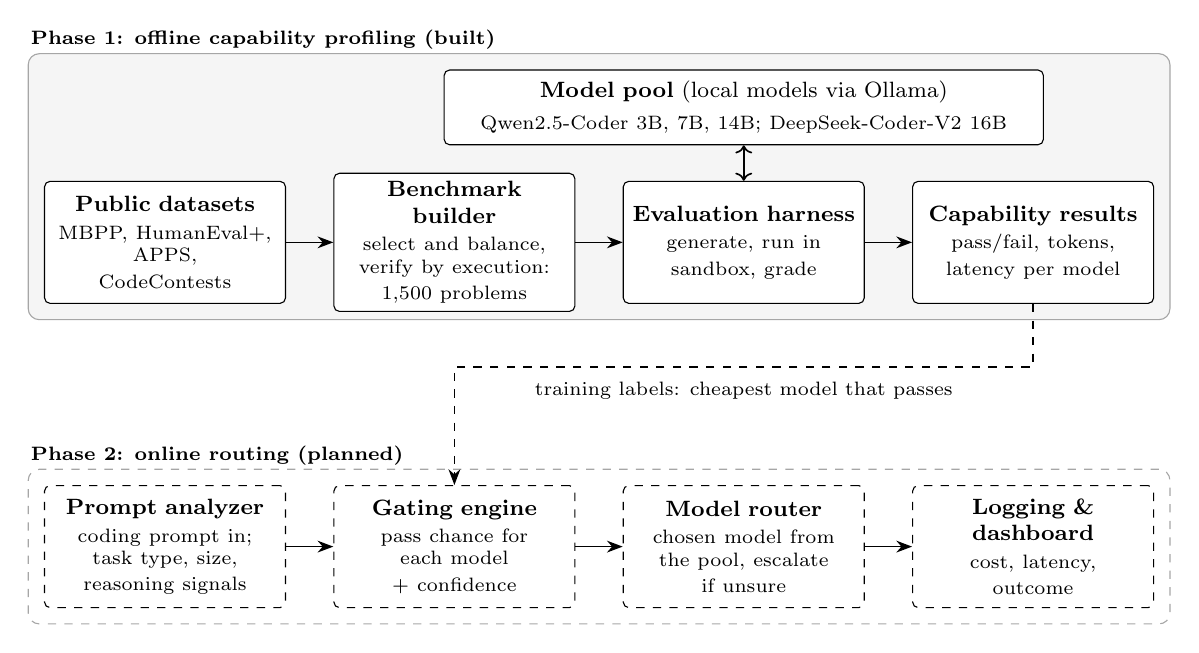
\begin{tikzpicture}[
  font=\footnotesize,
  box/.style={draw, rounded corners=2pt, align=center, text width=2.85cm,
              minimum height=1.55cm, fill=white, inner sep=3pt,
              execute at begin node={\hyphenpenalty=10000}},
  plan/.style={box, dashed},
  arr/.style={-{Stealth[length=2mm]}, semithick},
  node distance=0.6cm
]
% Phase 1 (built)
\node[box] (ds)  {\textbf{Public datasets}\\[2pt]\scriptsize MBPP, HumanEval+,\\ APPS,\\ CodeContests};
\node[box, right=of ds]  (bld) {\textbf{Benchmark builder}\\[2pt]\scriptsize select and balance,\\ verify by execution:\\ 1,500 problems};
\node[box, right=of bld] (ev)  {\textbf{Evaluation harness}\\[2pt]\scriptsize generate, run in\\ sandbox, grade};
\node[box, right=of ev]  (res) {\textbf{Capability results}\\[2pt]\scriptsize pass/fail, tokens,\\ latency per model};
\node[box, above=0.45cm of ev, text width=7.4cm, minimum height=0.95cm] (pool)
     {\textbf{Model pool} (local models via Ollama)\\[2pt]\scriptsize Qwen2.5-Coder 3B, 7B, 14B; DeepSeek-Coder-V2 16B};
\draw[arr] (ds) -- (bld);
\draw[arr] (bld) -- (ev);
\draw[arr] (ev) -- (res);
\draw[arr, <->] (pool) -- (ev);

% Phase 2 (planned)
\node[plan, below=2.3cm of ds]   (an)   {\textbf{Prompt analyzer}\\[2pt]\scriptsize coding prompt in;\\ task type, size,\\ reasoning signals};
\node[plan, right=of an]   (gate) {\textbf{Gating engine}\\[2pt]\scriptsize pass chance for\\ each model\\ + confidence};
\node[plan, right=of gate] (rt)   {\textbf{Model router}\\[2pt]\scriptsize chosen model from\\ the pool, escalate\\ if unsure};
\node[plan, right=of rt]   (log)  {\textbf{Logging \& dashboard}\\[2pt]\scriptsize cost, latency,\\ outcome};
\draw[arr] (an) -- (gate);
\draw[arr] (gate) -- (rt);
\draw[arr] (rt) -- (log);

% Link: results become training labels
\draw[arr, dashed] (res.south) -- ++(0,-0.8) -| (gate.north)
   node[pos=0.25, below=2pt, font=\scriptsize, align=center] {training labels: cheapest model that passes};

\begin{scope}[on background layer]
\node[fit=(ds)(res)(pool), draw=black!35, fill=black!4, rounded corners=4pt, inner sep=0.2cm,
      label={[anchor=south west, font=\scriptsize\bfseries, inner sep=1pt]north west:Phase 1: offline capability profiling (built)}] {};
\node[fit=(an)(log), draw=black!35, dashed, rounded corners=4pt, inner sep=0.2cm,
      label={[anchor=south west, font=\scriptsize\bfseries, inner sep=1pt]north west:Phase 2: online routing (planned)}] {};
\end{scope}
\end{tikzpicture}
\caption{SAGE architecture. Solid boxes are implemented; dashed boxes are planned. The capability results from Phase 1 become the training labels and evaluation baseline for the gating engine in Phase 2.}
\label{fig:arch}
\end{figure}

\paragraph{Phase 1: offline profiling (implemented).}
\begin{itemize}[leftmargin=*]
  \item \textbf{Benchmark builder.} Downloads four public datasets, selects and balances problems, runs each reference solution against its tests, and writes 1,500 verified problems to \code{coding_benchmark.jsonl}.
  \item \textbf{Evaluation harness.} For each (problem, model) pair, asks the model for a solution, runs it in an isolated process, grades it, and appends one result row.
  \item \textbf{Capability results.} \code{results.jsonl} holds one row per problem per model, with the verdict, the failure type, token counts and timings.
\end{itemize}

\paragraph{Phase 2: online routing (planned).}
\begin{itemize}[leftmargin=*]
  \item \textbf{Prompt analyzer.} Extracts cheap signals from the prompt: task type, input size, constraints, and signs that multi-step reasoning is needed.
  \item \textbf{Gating engine.} Predicts, for each model in the pool, how likely it is to solve the prompt, with a confidence score. It is trained on the capability results, which record exactly which models solved each problem.
  \item \textbf{Model router.} Sends the prompt to the chosen model in the pool (Qwen2.5-Coder 3B, 7B or 14B, or DeepSeek-Coder-V2). It escalates to a stronger model when confidence is low or when the answer fails a check.
  \item \textbf{Logging and dashboard.} Records the routing decision, tokens, latency and outcome of each request so that SAGE can be compared with baseline strategies.
\end{itemize}

Three design rules from the proposal guide both phases. The router must stay lightweight, so that its own cost does not cancel the savings. Model choices are configurable rather than hard-coded, because model prices and capabilities change. Every claim is backed by a measurable number: test pass rate, tokens and latency.

\subsection{Technical Stack}

\begin{itemize}[leftmargin=*]
  \item \textbf{Language:} Python~3.13 for the dataset build scripts and the evaluator. The evaluator is a single file that uses only the Python standard library. \code{numpy} is installed only because the official HumanEval+ test suites import it.
  \item \textbf{Data storage:} JSON Lines (\code{.jsonl}) for the benchmark and the results, and JSON for the dataset manifest, checker specifications and run summaries. Source data is loaded with the Hugging Face \code{datasets} library \cite{lhoest2021datasets} and stored as Parquet files.
  \item \textbf{Model serving:} Ollama \cite{ollama}, called through its local HTTP API (\code{/api/generate} on \code{localhost:11434}).
  \item \textbf{Models:} Qwen2.5-Coder 3B, 7B and 14B \cite{hui2024qwen25coder}, and DeepSeek-Coder-V2-Lite 16B \cite{deepseek2024coderv2}.
  \item \textbf{Tools:} the \code{test_evaluator.py} test suite, a 20-problem smoke test before every full run, and a re-scoring mode that re-grades stored answers without calling the model.
  \item \textbf{Hardware:} a Windows laptop with an NVIDIA RTX~4060 Laptop GPU (8~GB VRAM), Intel Core i7-14700HX and 15.7~GB RAM, and an Apple Silicon MacBook Air as a second machine.
  \item \textbf{Planned for Phase 2:} a lightweight classifier for the router, a backend framework for the routing gateway in front of Ollama, containerised deployment and a CI/CD pipeline, as described in the proposal.
\end{itemize}

\section{Implementation Details}

\subsection{Module 1: Benchmark Construction}

\paragraph{Sources.} No problems were written by hand. All 1,500 come from four established public benchmarks (Table~\ref{tab:sources}): MBPP \cite{austin2021mbpp}, HumanEval+ \cite{chen2021humaneval,liu2023evalplus}, APPS \cite{hendrycks2021apps} and CodeContests \cite{li2022alphacode}. They cover two task types:
\begin{itemize}[leftmargin=*]
  \item \textbf{Function tasks} (MBPP, HumanEval+). The model writes one Python function, which is graded by running assertions against it. HumanEval+ uses the official EvalPlus \code{check()} functions, which add many extra tests to the original HumanEval problems.
  \item \textbf{stdin/stdout tasks} (APPS, CodeContests). The model writes a complete program that reads standard input and prints to standard output. It is graded by comparing its output with the expected output for every test case.
\end{itemize}

\begin{table}[!htbp]
\centering
\small
\begin{tabular}{|l|l|r|L{2.7cm}|}
\hline
\textbf{Source} & \textbf{Hugging Face ID} & \textbf{Problems} & \textbf{Task type}\\
\hline
MBPP & \code{google-research-datasets/mbpp} & 387 & function\\
HumanEval+ & \code{evalplus/humanevalplus} & 163 & function\\
APPS & \code{codeparrot/apps} & 600 & stdin/stdout\\
CodeContests & \code{deepmind/code_contests} & 350 & stdin/stdout\\
\hline
\textbf{Total} & & \textbf{1,500} & 550 function + 950 stdin/stdout\\
\hline
\end{tabular}
\caption{Benchmark sources.}
\label{tab:sources}
\end{table}

\paragraph{Schema.} Each line of \code{coding_benchmark.jsonl} is one problem with exactly seven fields:

\begin{lstlisting}
{ "problem_id": "apps_0001",        "source": "apps",
  "task_type": "stdin_stdout",      "prompt": "problem statement ...",
  "tests": [ ... ],                 "reference_solution": "python source ...",
  "human_difficulty": "interview" }
\end{lstlisting}

For function tasks, \code{tests} holds Python assertion strings. For stdin/stdout tasks it holds \code{{"input": ..., "expected": ...}} pairs.

\paragraph{Difficulty labels.} We kept the labels the sources provide and did not invent any (Table~\ref{tab:difficulty}). APPS labels its problems introductory, interview or competition, and we map introductory to \emph{easy}. CodeContests gives a Codeforces rating, which we bucket into \emph{easy} (below 1300), \emph{medium} (1300--1699) and \emph{hard} (1700 and above); unrated problems are labelled \emph{competition}. MBPP and HumanEval+ have no labels, so their 550 problems are left as \code{null}.

\begin{table}[!htbp]
\centering
\small
\begin{tabular}{|l|r|l|}
\hline
\textbf{Difficulty} & \textbf{Count} & \textbf{Where it comes from}\\
\hline
\code{null} & 550 & MBPP + HumanEval+ (no labels in the source)\\
easy & 336 & APPS introductory (239) + CodeContests rating $<$ 1300 (97)\\
interview & 122 & APPS interview\\
competition & 302 & APPS competition (239) + unrated CodeContests (63)\\
medium & 63 & CodeContests rating 1300--1699\\
hard & 127 & CodeContests rating $\geq$ 1700\\
\hline
\end{tabular}
\caption{Difficulty distribution of the benchmark.}
\label{tab:difficulty}
\end{table}

\paragraph{Verification.} Every reference solution was executed against its own tests, and only problems whose reference passed were kept. Function references had to pass every assertion. For stdin/stdout problems, the reference was run on each test input and its output compared with the expected output after whitespace normalisation (Windows line endings converted, trailing spaces removed on each line, trailing blank lines dropped). This step also filters out most non-deterministic and special-judge problems, because a reference cannot reproduce a single fixed expected output for them. Each execution ran in a separate process with a timeout. \textbf{All 1,500 reference solutions pass their tests, with zero failures.}

\paragraph{Composition decisions.}
\begin{itemize}[leftmargin=*]
  \item HumanEval+ has 164 problems, not the 200 originally planned. The shortfall of 36 was moved to MBPP (350 $\rightarrow$ 387) instead of fabricating problems.
  \item \code{HumanEval/32} (\code{find_zero}) was excluded because it is a non-deterministic floating-point root finder (164 $\rightarrow$ 163).
  \item \code{mbpp_927}, \code{mbpp_180} and \code{mbpp_367} were excluded because their reference solutions fail their own official tests.
  \item APPS call-based problems were excluded by design, so APPS is used only for stdin/stdout. Because the APPS train split has few pure-stdin problems, introductory problems were also drawn from the APPS test split.
  \item For CodeContests, only official accepted Python~3 submissions were used as references. Problems come from the validation and test splits plus training shard~6, since validation and test alone gave only 282 usable problems.
\end{itemize}
The build is split into \code{build/assemble.py}, which selects and balances problems from each source, and \code{build/finalize.py}, which writes the final dataset together with \code{dataset_manifest.json} (counts, difficulty distribution, exclusions and validation summary).

\subsection{Module 2: Evaluation Harness}

The harness (\code{sage_evaluator/evaluator.py}) evaluates one problem at a time through the pipeline in Figure~\ref{fig:pipeline}.

\begin{figure}[htbp]
\centering
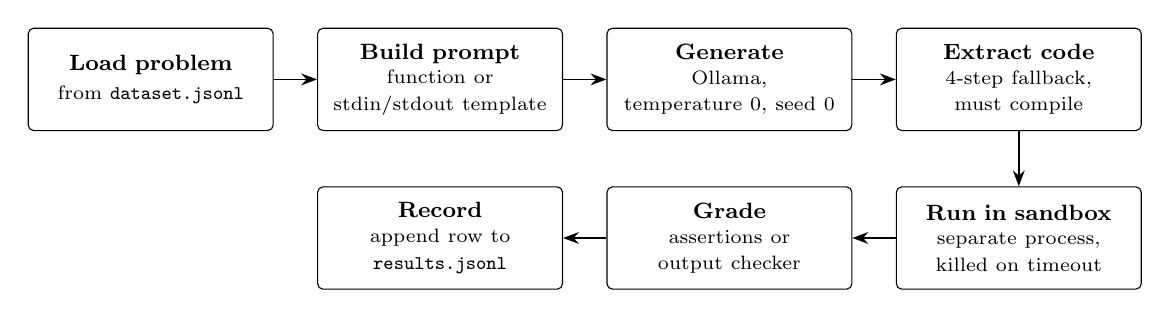
\begin{tikzpicture}[
  font=\footnotesize,
  stp/.style={draw, rounded corners=2pt, align=center, text width=2.9cm,
               minimum height=1.3cm, fill=white, inner sep=3pt},
  arr/.style={-{Stealth[length=2mm]}, semithick},
  node distance=0.55cm
]
\node[stp] (s1) {\textbf{Load problem}\\[1pt]\scriptsize from \texttt{dataset.jsonl}};
\node[stp, right=of s1] (s2) {\textbf{Build prompt}\\[1pt]\scriptsize function or\\ stdin/stdout template};
\node[stp, right=of s2] (s3) {\textbf{Generate}\\[1pt]\scriptsize Ollama,\\ temperature 0, seed 0};
\node[stp, right=of s3] (s4) {\textbf{Extract code}\\[1pt]\scriptsize 4-step fallback,\\ must compile};
\node[stp, below=0.7cm of s4] (s5) {\textbf{Run in sandbox}\\[1pt]\scriptsize separate process,\\ killed on timeout};
\node[stp, left=of s5] (s6) {\textbf{Grade}\\[1pt]\scriptsize assertions or\\ output checker};
\node[stp, left=of s6] (s7) {\textbf{Record}\\[1pt]\scriptsize append row to\\ \texttt{results.jsonl}};
\draw[arr] (s1) -- (s2);
\draw[arr] (s2) -- (s3);
\draw[arr] (s3) -- (s4);
\draw[arr] (s4) -- (s5);
\draw[arr] (s5) -- (s6);
\draw[arr] (s6) -- (s7);
\end{tikzpicture}
\caption{How the harness evaluates one problem with one model.}
\label{fig:pipeline}
\end{figure}

\paragraph{Prompting and generation.} The problem is wrapped in one of two prompt templates, one for function tasks and one for stdin/stdout programs, and sent to Ollama with temperature~0 and seed~0, so that re-running gives the same answer. Generation is bounded by a maximum number of output tokens (\code{--num-predict}, default 1024), a context window (\code{--num-ctx}, default 8192) and a time limit (\code{--gen-timeout}, default 600~s).

\paragraph{Code extraction.} Models wrap code in explanations and markdown, so the harness extracts it with four fallbacks, in order: (1) the first fenced \code{python} block that compiles; (2) the longest fenced block; (3) the whole response, if it compiles; (4) everything from the first line that looks like code, trimmed from the end until it compiles.

\paragraph{Sandboxed execution.} Candidate code runs in a separate worker process (\code{evaluator.py --_worker}) that is killed if it exceeds the execution timeout (30~s by default). Our first version ran candidate code in threads inside the evaluator. Python cannot kill a thread, so timed-out solutions kept running in the background and made every later test look like a timeout. Moving execution into killable subprocesses fixed this.

\paragraph{Grading.} The metric is \textbf{pass@1}: one attempt per problem, which passes only if \emph{all} its tests pass. Every result receives one of the statuses in Table~\ref{tab:status}.

\begin{table}[!htbp]
\centering
\small
\begin{tabular}{|L{3.9cm}|L{8.2cm}|}
\hline
\textbf{Status} & \textbf{Meaning}\\
\hline
\code{pass} & All tests passed\\
\code{wrong_answer} & A function assertion failed\\
\code{output_mismatch} & The stdin program ran but printed the wrong output\\
\code{runtime_error} & The code raised an exception\\
\code{syntax_error} & The code did not compile\\
\code{timeout} & Execution exceeded the timeout (30~s by default)\\
\code{no_code} & No code could be extracted from the response\\
\code{generation_error} & The Ollama call failed\\
\code{checker_error},\newline \code{checker_missing} & The checker could not judge the output (never counted as a pass)\\
\hline
\end{tabular}
\caption{Result statuses recorded by the harness.}
\label{tab:status}
\end{table}

\paragraph{Checker system.} Each result stores two verdicts. \code{strict_pass} is a normalised exact match against the expected output. \code{validated_pass} is the verdict of the problem's checker, and is identical to \code{strict_pass} unless a checker has been declared for that problem. The default checker is exact matching. Five problems whose statements explicitly allow a floating-point tolerance use a float checker. Each of these is listed in \code{checker_specs.json} together with the sentence from the statement that allows it. An automatic scan flagged 134 problems that may accept more than one valid output; these stay on strict checking until hand-written validators exist. An uncertain result is never counted as a pass, so the reported scores are, if anything, slight underestimates.

\paragraph{Recording and cost signals.} Each result is appended to \code{results.jsonl} and flushed to disk immediately. A row stores the verdict, tests passed out of total, the error type and message, the first failing test and the extracted code. It also stores run metadata: model name, generation and execution time, prompt and completion tokens, tokens per second, and every setting used. Token counts and generation time are the cost signals the router will optimise.

\paragraph{Operational features.} Problems already in the results file for a given model are skipped, so an interrupted run resumes where it stopped and \code{Ctrl+C} is safe. Several models share one results file, with every row tagged by model. Other options restrict a run to certain sources or to the first $N$ problems, print a summary of existing results, write the summary as JSON, and re-grade stored answers with a new checker configuration without calling the model again (\code{--rescore}).

\subsection{Module 3: Model Pool and Run Configuration}
\label{sec:models}

\paragraph{Why local open-source models.} SAGE's router chooses between open-source code models served locally. We chose this setup for three reasons:
\begin{enumerate}[leftmargin=*]
  \item \textbf{Cost.} One full profile is 1,500 model calls. Running several profiles on paid APIs would be expensive, and every bug fix in the harness would mean paying again. Local models cost nothing per call.
  \item \textbf{Reproducibility.} Local models with temperature~0 and a fixed seed give the same output on every run. Results can be re-graded and audited without regenerating them.
  \item \textbf{A clean tier ladder, plus a second family.} The core of the pool is one model family, Qwen2.5-Coder \cite{hui2024qwen25coder}, at three sizes. All three share the same training recipe and prompt format, so differences between them come from model size alone. This gives the router a real cost ladder: a small, fast, cheap model, a mid-sized one, and a larger, slower, stronger one. We add DeepSeek-Coder-V2-Lite \cite{deepseek2024coderv2} from a different family. It is a mixture-of-experts model: it has 16B parameters in total but uses only about 2.4B of them for each token it generates. It shows whether models of similar size from different families are good at different things, which matters for routing.
\end{enumerate}
All four models are non-reasoning code models: they write code directly, with no separate ``thinking'' step.

\begin{table}[!htbp]
\centering
\small
\begin{tabular}{|l|l|r|l|l|}
\hline
\textbf{Model} & \textbf{Ollama tag} & \textbf{Size} & \textbf{Role} & \textbf{Status}\\
\hline
Qwen2.5-Coder 3B & \code{qwen2.5-coder:3b} & 1.9~GB & cheap & complete\\
Qwen2.5-Coder 7B & \code{qwen2.5-coder:7b} & 4.7~GB & mid & complete\\
Qwen2.5-Coder 14B & \code{qwen2.5-coder:14b} & 9.0~GB & strong & complete\\
DeepSeek-Coder-V2 16B & \code{deepseek-coder-v2:16b} & 8.9~GB & 2nd family & complete\\
\hline
\end{tabular}
\caption{Models in the study (size is the Ollama download). In later tables, ``DS-V2'' is DeepSeek-Coder-V2-Lite 16B.}
\label{tab:models}
\end{table}

\paragraph{Run settings.} All runs use temperature~0, seed~0 and a 30~s execution timeout (Table~\ref{tab:settings}). The output and context limits differ between models: the 7B and 14B share the same limits, the 3B used a larger output limit and a smaller context, and DeepSeek-Coder-V2 was run with the largest limits on a second machine. No prompt exceeded any model's context window (the longest prompt is 3,774 tokens), and three of the four models almost never hit their output limit, so the different limits did not change their results. The Qwen 14B hit its limit far more often, almost always because of the repetition loops described in Section~\ref{sec:analysis}. Its download (9.0~GB) is also larger than the laptop GPU's 8~GB of memory, so it cannot run entirely on that GPU.

\begin{table}[!htbp]
\centering
\small
\begin{tabular}{|l|r|r|r|}
\hline
\textbf{Model} & \textbf{Max output} & \textbf{Context} & \textbf{Output-limit hits}\\
\hline
Qwen2.5-Coder 3B & 4,096 & 4,096 & 12\\
Qwen2.5-Coder 7B & 1,024 & 8,192 & 13\\
Qwen2.5-Coder 14B & 1,024 & 8,192 & 218\\
DeepSeek-Coder-V2-Lite 16B & 8,192 & 16,384 & 1\\
\hline
\end{tabular}
\caption{Generation settings per model, in tokens. Of the Qwen 14B's 218 output-limit hits, 168 are repetition loops and 50 are long answers cut off at 1,024 tokens.}
\label{tab:settings}
\end{table}

% =====================================================================
\chapter{Results and Evaluation}
% =====================================================================

\section{Testing Methodology}

\begin{itemize}[leftmargin=*]
  \item \textbf{Unit Testing:} \code{test_evaluator.py} tests the evaluator and the checker system (\code{checkers.py}, which provides exact, token, float, special-judge and optimisation checkers). The example special-judge and optimisation validators in \code{validators/} exist only for these tests.
  \item \textbf{Integration Testing:} The reference-solution check is an end-to-end test of the grading path: all 1,500 reference solutions go through the same execution and comparison logic as model answers, and all of them pass. This shows that the tests, the output normalisation and the sandbox agree with each other. Before every full run, a 20-problem smoke test checks the model, the machine and the settings together. After any environment change, stored answers are re-graded with \code{--rescore} instead of regenerated; this is how the DeepSeek-Coder-V2 HumanEval+ results were re-graded after \code{numpy} was installed on its machine.
  \item \textbf{Performance Testing:} Every result row records generation time, execution time, output tokens and tokens per second. We use these to estimate how long a full run of a larger model will take on our hardware and to compare models by output length.
  \item \textbf{Result Validity Audit:} There are no end users at this stage, so in place of user testing we audited the results for evaluator bugs. The HumanEval+ scores of all four models (Qwen 79.8\%, 84.7\% and 85.9\%; DeepSeek-Coder-V2 73.6\%) are consistent with the published results for these models. For the Qwen 7B, none of the wrong stdin/stdout answers were formatting near-misses, no non-Python code appeared, and 98\% of stdin/stdout solutions read the input correctly. We also inspected every answer that hit the output limit, which is how the Qwen 14B's repetition loops were found. The low stdin/stdout scores therefore reflect the models, not the harness.
\end{itemize}

\section{Performance Metrics}

Table~\ref{tab:goals} compares the mid-semester goals with what was achieved.

\begin{table}[!htbp]
\centering
\small
\begin{tabular}{|L{3.4cm}|L{4.3cm}|L{4.6cm}|}
\hline
\textbf{Goal} & \textbf{Target} & \textbf{Achieved}\\
\hline
Benchmark size & 1,500 problems from public sources & 1,500 from 4 sources (550 function + 950 stdin/stdout)\\
Reference verification & 100\% of references pass & 1,500 / 1,500 (0 failures)\\
Reproducible evaluation & Deterministic, sandboxed, resumable & Done: temperature 0, seed 0, killable subprocess, fsync'd rows\\
Model profiles & Qwen2.5-Coder 3B, 7B, 14B and DeepSeek-Coder-V2-Lite $\times$ 1,500 problems & All four complete (6,000 graded answers)\\
Gating engine & End-semester & Not started (Phase 2)\\
\hline
\end{tabular}
\caption{Mid-semester goals and status.}
\label{tab:goals}
\end{table}

Table~\ref{tab:results} and Figure~\ref{fig:bysource} give pass@1 on all 1,500 problems.

\begin{table}[!htbp]
\centering
\small
\setlength{\tabcolsep}{4pt}
\begin{tabular}{|l|r|r|r|r|}
\hline
 & \textbf{Qwen 3B} & \textbf{Qwen 7B} & \textbf{Qwen 14B} & \textbf{DS-V2 16B}\\
\hline
\textbf{Overall (1,500)} & 507 (33.8\%) & 606 (40.4\%) & \textbf{678 (45.2\%)} & 628 (41.9\%)\\
\hline
MBPP (387) & 239 (61.8\%) & 304 (78.6\%) & \textbf{327 (84.5\%)} & 280 (72.4\%)\\
HumanEval+ (163) & 130 (79.8\%) & 138 (84.7\%) & \textbf{140 (85.9\%)} & 120 (73.6\%)\\
APPS (600) & 107 (17.8\%) & 126 (21.0\%) & 156 (26.0\%) & \textbf{173 (28.8\%)}\\
CodeContests (350) & 31 (8.9\%) & 38 (10.9\%) & \textbf{55 (15.7\%)} & \textbf{55 (15.7\%)}\\
\hline
Function (550) & 369 (67.1\%) & 442 (80.4\%) & \textbf{467 (84.9\%)} & 400 (72.7\%)\\
stdin/stdout (950) & 138 (14.5\%) & 164 (17.3\%) & 211 (22.2\%) & \textbf{228 (24.0\%)}\\
\hline
\end{tabular}
\caption{pass@1 by source and task type (problems solved and percentage). Bold marks the best model in each row.}
\label{tab:results}
\end{table}

\begin{figure}[htbp]
\centering
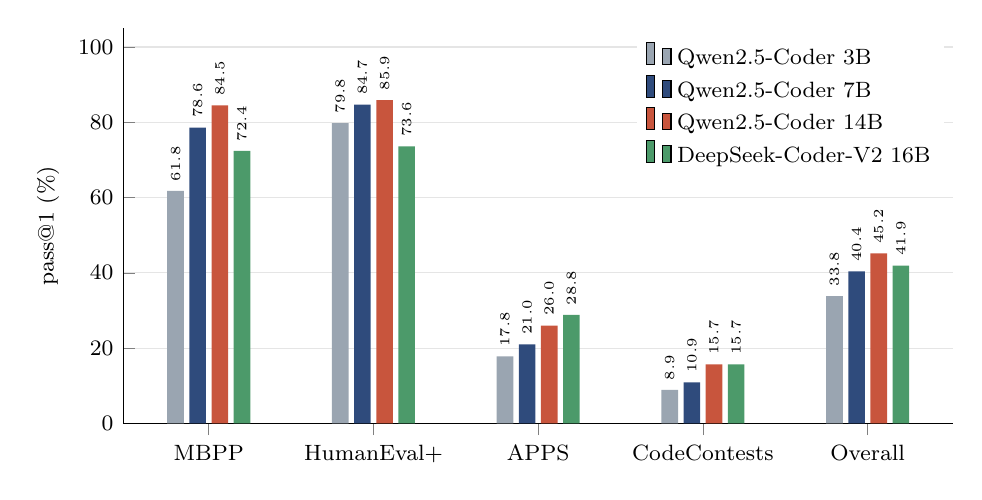
\begin{tikzpicture}
\begin{axis}[
  ybar, bar width=6pt, width=\textwidth, height=6.6cm,
  ymin=0, ymax=105, ylabel={pass@1 (\%)},
  symbolic x coords={MBPP,HumanEval+,APPS,CodeContests,Overall},
  xtick=data, enlarge x limits=0.13,
  nodes near coords, every node near coord/.append style={font=\tiny, rotate=90, anchor=west,
     /pgf/number format/fixed, /pgf/number format/fixed zerofill, /pgf/number format/precision=1},
  axis lines*=left, ymajorgrids, grid style={black!10},
  tick label style={font=\footnotesize}, label style={font=\footnotesize},
  legend style={at={(0.99,0.98)}, anchor=north east, font=\footnotesize, draw=none, fill=white},
  legend cell align=left
]
\addplot[fill=q3b, draw=none] coordinates {(MBPP,61.8) (HumanEval+,79.8) (APPS,17.8) (CodeContests,8.9) (Overall,33.8)};
\addplot[fill=q7b, draw=none] coordinates {(MBPP,78.6) (HumanEval+,84.7) (APPS,21.0) (CodeContests,10.9) (Overall,40.4)};
\addplot[fill=q14b, draw=none] coordinates {(MBPP,84.5) (HumanEval+,85.9) (APPS,26.0) (CodeContests,15.7) (Overall,45.2)};
\addplot[fill=dsv2, draw=none] coordinates {(MBPP,72.4) (HumanEval+,73.6) (APPS,28.8) (CodeContests,15.7) (Overall,41.9)};
\legend{Qwen2.5-Coder 3B, Qwen2.5-Coder 7B, Qwen2.5-Coder 14B, DeepSeek-Coder-V2 16B}
\end{axis}
\end{tikzpicture}
\caption{pass@1 by source. Within Qwen, scores rise with size on every source. DeepSeek-Coder-V2 trails the Qwen 7B and 14B on the function benchmarks but leads on APPS.}
\label{fig:bysource}
\end{figure}

For the 950 stdin/stdout problems, which carry difficulty labels, Table~\ref{tab:bydiff} and Figure~\ref{fig:bydiff} break the result down by difficulty.

\begin{table}[!htbp]
\centering
\small
\setlength{\tabcolsep}{4pt}
\begin{tabular}{|l|r|r|r|r|}
\hline
\textbf{Difficulty} & \textbf{Qwen 3B} & \textbf{Qwen 7B} & \textbf{Qwen 14B} & \textbf{DS-V2 16B}\\
\hline
easy (336) & 91 (27.1\%) & 113 (33.6\%) & 141 (42.0\%) & \textbf{146 (43.5\%)}\\
interview (122) & 10 (8.2\%) & 11 (9.0\%) & \textbf{22 (18.0\%)} & 18 (14.8\%)\\
medium (63) & 6 (9.5\%) & 5 (7.9\%) & 5 (7.9\%) & \textbf{10 (15.9\%)}\\
hard (127) & 3 (2.4\%) & 2 (1.6\%) & 2 (1.6\%) & \textbf{9 (7.1\%)}\\
competition (302) & 28 (9.3\%) & 33 (10.9\%) & 41 (13.6\%) & \textbf{45 (14.9\%)}\\
\hline
\end{tabular}
\caption{pass@1 on stdin/stdout problems by difficulty label. MBPP and HumanEval+ have no difficulty labels. Bold marks the best model in each row.}
\label{tab:bydiff}
\end{table}

\begin{figure}[htbp]
\centering
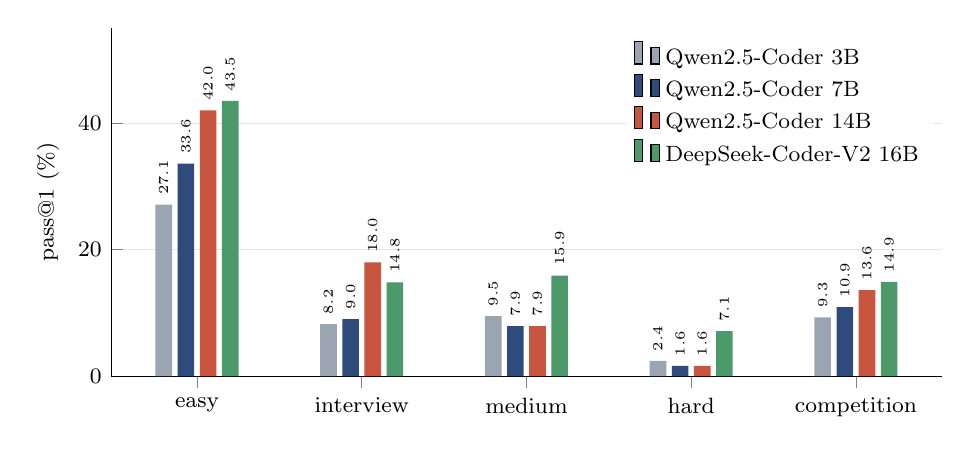
\begin{tikzpicture}
\begin{axis}[
  ybar, bar width=6pt, width=\textwidth, height=6cm,
  ymin=0, ymax=55, ylabel={pass@1 (\%)},
  symbolic x coords={easy,interview,medium,hard,competition},
  xtick=data, enlarge x limits=0.13,
  nodes near coords, every node near coord/.append style={font=\tiny, rotate=90, anchor=west,
     /pgf/number format/fixed, /pgf/number format/fixed zerofill, /pgf/number format/precision=1},
  axis lines*=left, ymajorgrids, grid style={black!10},
  tick label style={font=\footnotesize}, label style={font=\footnotesize},
  legend style={at={(0.99,0.98)}, anchor=north east, font=\footnotesize, draw=none, fill=white},
  legend cell align=left
]
\addplot[fill=q3b, draw=none] coordinates {(easy,27.1) (interview,8.2) (medium,9.5) (hard,2.4) (competition,9.3)};
\addplot[fill=q7b, draw=none] coordinates {(easy,33.6) (interview,9.0) (medium,7.9) (hard,1.6) (competition,10.9)};
\addplot[fill=q14b, draw=none] coordinates {(easy,42.0) (interview,18.0) (medium,7.9) (hard,1.6) (competition,13.6)};
\addplot[fill=dsv2, draw=none] coordinates {(easy,43.5) (interview,14.8) (medium,15.9) (hard,7.1) (competition,14.9)};
\legend{Qwen2.5-Coder 3B, Qwen2.5-Coder 7B, Qwen2.5-Coder 14B, DeepSeek-Coder-V2 16B}
\end{axis}
\end{tikzpicture}
\caption{pass@1 on stdin/stdout problems by difficulty. All three Qwen sizes are flat on medium and hard problems; DeepSeek-Coder-V2 is the only model that makes progress there.}
\label{fig:bydiff}
\end{figure}

Table~\ref{tab:failures} shows how the failures are distributed, and Table~\ref{tab:gen} compares how much each model writes.

\begin{table}[!htbp]
\centering
\small
\begin{tabular}{|l|r|r|r|r|}
\hline
\textbf{Status} & \textbf{Qwen 3B} & \textbf{Qwen 7B} & \textbf{Qwen 14B} & \textbf{DS-V2 16B}\\
\hline
\code{pass} & 507 & 606 & 678 & 628\\
\code{output_mismatch} & 617 & 648 & 663 & 611\\
\code{runtime_error} & 209 & 114 & 65 & 172\\
\code{wrong_answer} & 134 & 100 & 72 & 54\\
\code{timeout} & 31 & 32 & 22 & 31\\
\code{syntax_error} & 2 & 0 & 0 & 4\\
\hline
\textbf{Total} & 1,500 & 1,500 & 1,500 & 1,500\\
\hline
\end{tabular}
\caption{Result status counts over all 1,500 problems. Some models copy the example assertions from the prompt into their own code; when their function is wrong, that copied assertion fails first and is recorded as a \code{runtime_error} instead of a \code{wrong_answer} (82 cases for DeepSeek-Coder-V2 and 22 for the Qwen 3B, all on MBPP). The problem fails either way, so pass rates are unaffected.}
\label{tab:failures}
\end{table}

\begin{table}[!htbp]
\centering
\small
\begin{tabular}{|l|r|r|r|r|}
\hline
 & \textbf{Qwen 3B} & \textbf{Qwen 7B} & \textbf{Qwen 14B} & \textbf{DS-V2 16B}\\
\hline
Median output tokens & 214 & 115 & 171 & 160\\
Total output tokens & 498,354 & 215,441 & 442,896 & 287,146\\
Mean generation time & 5.36~s & 3.23~s & 30.33~s & 4.15~s\\
Repetition loops & 0 & 0 & 168 & 1\\
\hline
\end{tabular}
\caption{Generation statistics per problem (total tokens over all 1,500). The models ran on different machines, so their times are not directly comparable.}
\label{tab:gen}
\end{table}

\section{Analysis}
\label{sec:analysis}

\paragraph{Did we meet our objectives?} Objectives 1 and 2 are fully met: the benchmark has 1,500 problems with every reference verified, and the harness is deterministic, sandboxed and resumable. Objective 3 is met: the three-model Qwen ladder and DeepSeek-Coder-V2 have all been run on all 1,500 problems, giving 6,000 graded answers. The overall ranking is Qwen 14B (45.2\%), DeepSeek-Coder-V2 (41.9\%), Qwen 7B (40.4\%) and Qwen 3B (33.8\%). The results say several things that matter for the router.

\paragraph{1. Within one family, performance rises steadily with size.} The Qwen pass rate goes from 33.8\% (3B) to 40.4\% (7B) to 45.2\% (14B): 99 more problems from 3B to 7B, and 72 more from 7B to 14B. The models also make fewer basic mistakes as they grow. Runtime errors fall from 209 to 114 to 65, and failed assertions from 134 to 100 to 72.

\paragraph{2. Where the gains come from changes with size.} From 3B to 7B the improvement is mostly on function tasks (+13.3 points, and +16.8 on MBPP). From 7B to 14B function tasks gain less (+4.5 points), because they are close to a ceiling of about 85\%: the 14B scores 84.5\% on MBPP and 85.9\% on HumanEval+, only 1.2 points above the 7B on HumanEval+. Instead, the 14B gains more on stdin/stdout problems (+4.9 points against +2.7 for the previous step), especially easy problems (33.6\% to 42.0\%) and interview problems (9.0\% to 18.0\%). For the router, this means the extra cost of the 14B buys little on short function tasks but measurably more on algorithmic ones.

\paragraph{3. Different families have different strengths.} DeepSeek-Coder-V2 and the Qwen 14B are close in overall score, but they are good at different things (Table~\ref{tab:h2h}). Qwen is clearly better at writing functions: the 14B solves 92 function problems that DeepSeek misses, against 25 the other way. DeepSeek is better on stdin/stdout algorithmic problems (24.0\% against 22.2\%), and it is the only model that makes real progress on the hardest problems: 10 of 63 medium and 9 of 127 hard problems, against 5 and 2 for the Qwen 14B. It is also efficient: with only about 2.4B parameters active per token, it beats the dense Qwen 7B overall. Part of the Qwen 14B's stdin/stdout gap is caused by its repetition loops (point~7), so its true algorithmic ability may be close to DeepSeek's. Even so, a router that can choose across families has options a single-family ladder does not.

\begin{table}[!htbp]
\centering
\small
\begin{tabular}{|l|r|r|r|}
\hline
 & \textbf{Function (550)} & \textbf{stdin/stdout (950)} & \textbf{Total (1,500)}\\
\hline
Only Qwen 14B & 92 & 73 & 165\\
Only DeepSeek-Coder-V2 & 25 & 90 & 115\\
\hline
\end{tabular}
\caption{Problems solved by only one of the Qwen 14B and DeepSeek-Coder-V2. Of the remaining problems, 513 are solved by both and 707 by neither.}
\label{tab:h2h}
\end{table}

\paragraph{4. Some problems are out of reach for every model.} 664 problems (44.3\%) are solved by none of the four models, and medium and hard problems stay mostly unsolved by all of them. A router choosing only among these models cannot help on these problems. They would need a stronger model, such as a reasoning model that plans before writing code; for the router, the sensible choice on such prompts is the cheapest model, since no model in the pool is likely to succeed. Difficulty labels also do not line up across sources: for the Qwen 3B and 7B, APPS ``interview'' problems were solved less often than ``competition'' problems. The router therefore has to estimate difficulty from the prompt itself, using measured pass/fail outcomes as ground truth.

\paragraph{5. Most of what a large model solves, a smaller model also solves.} Table~\ref{tab:overlap} shows which combination of Qwen models solved each problem. Of the 678 problems the Qwen 14B solves, 461 (68\%) are also solved by the 3B, and 573 (85\%) by the 3B or the 7B. Only 105 problems are solved by the 14B alone among the Qwen models. A larger model is also not better on every problem: 91 problems are solved by the 3B or the 7B but not by the 14B. Across all four models, 386 problems are solved by every model, and each model solves some problems no other model does (3B: 12, 7B: 25, 14B: 68, DeepSeek: 67). This is why the router should predict, for each model separately, whether it will pass, rather than placing each problem on a single difficulty scale.

\begin{table}[!htbp]
\centering
\small
\begin{tabular}{|l|c|c|c|r|}
\hline
 & \multicolumn{3}{c|}{\textbf{Solved by}} & \\
\cline{2-4}
\textbf{Which models solved it} & \textbf{3B} & \textbf{7B} & \textbf{14B} & \textbf{Problems}\\
\hline
All three & Yes & Yes & Yes & 432\\
7B and 14B only & -- & Yes & Yes & 112\\
14B only & -- & -- & Yes & 105\\
3B and 14B only & Yes & -- & Yes & 29\\
3B and 7B only & Yes & Yes & -- & 17\\
7B only & -- & Yes & -- & 45\\
3B only & Yes & -- & -- & 29\\
None of the three & -- & -- & -- & 731\\
\hline
\multicolumn{4}{|l|}{\textbf{Total}} & 1,500\\
\hline
\end{tabular}
\caption{Problem overlap across the three Qwen2.5-Coder models. Each row counts the problems solved by exactly that combination of models: ``Yes'' means the model passed all tests for the problem, ``--'' means it failed.}
\label{tab:overlap}
\end{table}

\paragraph{6. Routing headroom.} Table~\ref{tab:rule} compares routing strategies, using the share of requests sent to each model as a simple cost measure. A perfect (``oracle'') router that knew in advance which models would pass would send each problem to the cheapest Qwen model that solves it, to DeepSeek-Coder-V2 only when no Qwen model does, and to the 3B when no model does. It would solve 836 problems (55.7\%), 158 more than always using the Qwen 14B, while sending 78\% of requests to the 3B and only 7\% to the 14B. This is an upper bound computed with hindsight, not an achievable result, but it shows how much room a router has. Simple rules based on task type already help. Sending function tasks to the Qwen 14B and stdin/stdout tasks to DeepSeek-Coder-V2 solves 695 problems, more than any single model. Sending function tasks to the cheaper Qwen 7B instead still solves 670. These rules were chosen after seeing the results, so they are in-sample illustrations; the learned router must beat them on held-out problems.

\begin{table}[!htbp]
\centering
\small
\setlength{\tabcolsep}{4pt}
\begin{tabular}{|l|r|r|r|r|r|}
\hline
\textbf{Strategy} & \textbf{Solved} & \textbf{3B} & \textbf{7B} & \textbf{14B} & \textbf{DS-V2}\\
\hline
Always Qwen 3B & 507 (33.8\%) & 100\% & -- & -- & --\\
Always Qwen 7B & 606 (40.4\%) & -- & 100\% & -- & --\\
Always Qwen 14B & 678 (45.2\%) & -- & -- & 100\% & --\\
Always DS-V2 & 628 (41.9\%) & -- & -- & -- & 100\%\\
Function $\rightarrow$ 7B, stdin $\rightarrow$ 14B & 653 (43.5\%) & -- & 36.7\% & 63.3\% & --\\
Function $\rightarrow$ 7B, stdin $\rightarrow$ DS-V2 & 670 (44.7\%) & -- & 36.7\% & -- & 63.3\%\\
Function $\rightarrow$ 14B, stdin $\rightarrow$ DS-V2 & 695 (46.3\%) & -- & -- & 36.7\% & 63.3\%\\
Oracle (hindsight upper bound) & 836 (55.7\%) & 78.1\% & 10.5\% & 7.0\% & 4.5\%\\
\hline
\end{tabular}
\caption{Routing strategies across the four models, with the share of requests sent to each (computed from Tables~\ref{tab:results} and \ref{tab:overlap} and the four-model overlap counts).}
\label{tab:rule}
\end{table}

\paragraph{7. The Qwen 14B falls into repetition loops.} On 168 stdin/stdout problems (17.7\% of them: 100 from APPS and 68 from CodeContests), the Qwen 14B started a solution and then repeated the same line, almost always \code{import sys}, until it ran out of tokens. No working program was produced, so all 168 count as failures. The other models had at most one such loop. This is a known weakness of greedy (temperature~0) decoding, so the 14B's stdin/stdout score of 22.2\% is a lower bound on its real ability. Excluding the loop cases, its stdin/stdout pass rate would be 27.0\% (211 of 782). That figure is only indicative, because the loop cases may be harder than average, and the official score remains 22.2\%.

\paragraph{8. Cost is not the same as size.} The Qwen 3B wrote more output tokens than the 7B (median 214 against 115 per problem, and 2.3 times as many in total). The Qwen 14B's total (442,896 tokens) is inflated by its repetition loops, each of which ran to the 1,024-token limit. DeepSeek-Coder-V2 has more parameters in total than any Qwen model, but it uses only about 2.4B of them for each token, so it runs fast for its size. Cost per request depends on the number of tokens as well as the price per token, so the router's cost model must use measured tokens multiplied by each model's price, not just the number of requests or the parameter count.

\paragraph{Challenges and how we resolved them.} Table~\ref{tab:issues} lists the main problems met so far.

\begin{table}[!htbp]
\centering
\small
\begin{tabular}{|L{3.4cm}|L{3.9cm}|L{5.4cm}|}
\hline
\textbf{Problem} & \textbf{Cause} & \textbf{Fix}\\
\hline
APPS and CodeContests would not load & \code{datasets} 5.x dropped support for loading scripts & Load the auto-converted Parquet mirror (\code{refs/convert/parquet})\\
Large downloads silently corrupted & OneDrive truncates large synced files & Download to a non-synced temporary folder\\
Every test started timing out during verification & In-process timeouts left threads running in the background & Run each execution in a killable subprocess\\
\code{ValueError}: integer exceeds 4,300 digits & Huge integers in APPS tests (Python~3.13 limit) & Raise the limit with \code{sys.set_int_max_str_digits}\allowbreak\code{(1000000)}\\
Model downloads stalled & Cloudflare WARP full-tunnel mode broke long downloads & Disconnect WARP while pulling models\\
DeepSeek-Coder-V2 scored 0\% on HumanEval+ & The test suites import \code{numpy}, which was not installed on its machine & Install \code{numpy}, then re-grade the stored answers with \code{--rescore}\\
The Qwen 14B does not fit on the laptop GPU & 8~GB of GPU memory; the 14B download alone is 9.0~GB & Accept slower generation (about 30~s per problem); the harness resumes interrupted runs\\
Qwen 14B repetition loops on 168 problems & Greedy decoding gets stuck repeating one line & Found by inspecting output-limit hits; reported separately for now (fix planned, see Section~\ref{sec:future})\\
\hline
\end{tabular}
\caption{Problems met and how they were handled.}
\label{tab:issues}
\end{table}

\paragraph{Threats to validity.} pass@1 uses a single deterministic sample, so it does not capture how often a model succeeds when sampled several times; a problem near a model's ability limit may pass or fail by chance. The same greedy decoding caused the Qwen 14B's repetition loops, which lower its stdin/stdout score. MBPP and HumanEval are widely published, so the models may have seen these problems during training, which could inflate their function-task scores. The 134 possibly multi-answer problems are checked strictly, which can only lower the scores. Finally, the models used different output and context limits and ran on different machines. The limits rarely came into play, but timings are not directly comparable, so cost comparisons should use token counts rather than seconds.

% =====================================================================
\chapter{Conclusion}
% =====================================================================

\section{Summary of Work}

In the first half of the semester we built the measurement foundation that the SAGE router depends on. We assembled a 1,500-problem Python benchmark from MBPP, HumanEval+, APPS and CodeContests, keeping only problems whose reference solutions pass their own tests (all 1,500 do). We built an evaluation harness that queries a model, extracts its code, runs it in a killable sandbox, grades it, and records the outcome together with token and time costs. With it we profiled four models on the full benchmark: a three-tier Qwen2.5-Coder ladder (3B, 7B, 14B) and DeepSeek-Coder-V2-Lite 16B from a second model family. Objectives 1, 2 and 3 are complete, and Objective 4, the router itself, is the work of the second half.

\section{Key Findings}

\begin{itemize}[leftmargin=*]
  \item \textbf{Finding 1:} Within the Qwen family, performance rises steadily with size, from 33.8\% (3B) to 40.4\% (7B) to 45.2\% (14B). The 3B-to-7B step helps mostly on function tasks; the 7B-to-14B step helps more on algorithmic stdin/stdout tasks, because function tasks are close to a ceiling.
  \item \textbf{Finding 2:} Model families have different strengths. Qwen is better at function tasks, while DeepSeek-Coder-V2 is better on stdin/stdout problems and is the only model that makes progress on medium and hard ones. Routing function tasks to the Qwen 14B and stdin/stdout tasks to DeepSeek beats every single model (695 against 678 problems, in-sample).
  \item \textbf{Finding 3:} Smaller models already cover most of what larger ones solve: 85\% of the Qwen 14B's solved problems are also solved by the 3B or 7B. A hindsight oracle across the four models would solve 836 problems (55.7\%) while sending 78\% of requests to the 3B. This is the headroom SAGE aims to capture.
  \item \textbf{Finding 4:} 664 problems (44.3\%) are solved by none of the four models, and no model in the pool helps on them; the router should send such prompts to the cheapest model rather than waste the most expensive one. Cost and quality must be measured per model, in tokens and pass rate, not assumed from model size: the Qwen 14B looped on 17.7\% of stdin/stdout problems, and the 3B wrote more tokens than the 7B.
\end{itemize}

\section{Future Work and Recommendations}
\label{sec:future}

\paragraph{Objective for the second half.} Build SAGE's gating router for the four models profiled in this report. Given a new coding prompt, the router predicts which of Qwen2.5-Coder 3B, 7B, 14B and DeepSeek-Coder-V2 will solve it, and sends it to the cheapest model likely to succeed. Success means solving close to as many problems as always using the strongest model (the Qwen 14B, 45.2\%), while sending most prompts to the cheaper models and using measurably fewer tokens and less compute. The router is trained on the 6,000 graded answers collected so far and tested on problems it has not seen.

The steps to get there are:
\begin{enumerate}[leftmargin=*]
  \item \textbf{Fix the repetition loops.} Re-run the 168 looping problems for the Qwen 14B with a repetition penalty or a small sampling temperature, or detect loops and retry, and report the corrected score next to the original one.
  \item \textbf{Build routing labels and baselines.} For every problem, record which models pass and the cheapest one that does. From these labels, compute the oracle router and the always-strongest, always-cheapest and task-type-rule baselines, measuring cost in tokens.
  \item \textbf{Train and evaluate the gating engine.} Extract lightweight features from the prompt text (task type, length, input constraints, presence of examples), train a model that predicts, for each model, whether it will pass, and route to the cheapest model predicted to succeed. Evaluate it on held-out problems against the baselines above.
  \item \textbf{Add confidence-aware escalation.} Send low-confidence prompts to a stronger model directly, and retry failed answers on a stronger model, measuring how often escalation is needed.
  \item \textbf{Deploy the gateway.} Build the routing API in front of the Ollama models, with logging and a dashboard showing model usage, estimated savings, routing accuracy and failure cases, with CI running unit and routing tests on every change.
  \item \textbf{Improve grading.} Write validators for the 134 possibly multi-answer problems so that correct alternative outputs are counted.
\end{enumerate}

\section{Final Remarks}

The main lesson of this phase is that a router is only as good as the data it learns from. Building a trustworthy benchmark and harness took longer than expected, mostly because of failures that had nothing to do with models: corrupted downloads, threads that could not be killed, missing libraries, and a large model silently repeating itself. Fixing or exposing these gave us results we can defend. Those results show that bigger models solve more, that smaller models already handle most of the same problems, and that models from different families are good at different things, so no single model is best everywhere. These facts are the reason SAGE exists. The second half of the semester turns this measured evidence into a working router and tests whether it can cut cost while keeping coding quality close to the strongest model.

% =====================================================================
\clearpage
\phantomsection
\addcontentsline{toc}{chapter}{Bibliography}
\bibliographystyle{alpha}
\bibliography{sage_refs}

\end{document}
